\documentclass[12pt]{article}
\setlength\parindent{0pt}
\usepackage{fullpage}
\usepackage{epsf}
\usepackage{enumerate}
\usepackage{amsmath}
\usepackage{graphicx}
\usepackage{enumitem}
\usepackage[margin=0.7in]{geometry}
\setlength{\parskip}{4mm}
\def\BS{\bigskip} 
\def\LL{\left\langle}   % left angle bracket
\def\RR{\right\rangle}  % right angle bracket
\def\LP{\left(}         % left parenthesis
\def\RP{\right)}        % right parenthesis
\def\LB{\left\{}        % left curly bracket
\def\RB{\right\}}       % right curly bracket
\def\PAR#1#2{ {{\partial #1}\over{\partial #2}} }
\def\PARTWO#1#2{ {{\partial^2 #1}\over{\partial #2}^2} }
\def\PARTWOMIX#1#2#3{ {{\partial^2 #1}\over{\partial #2 \partial #3}} }
\newcommand{\BC}{\begin{center}}
\newcommand{\EC}{\end{center}}
\newcommand{\BE}{\begin{displaymath}}
\newcommand{\EE}{\end{displaymath}}
\newcommand{\BNE}{\begin{equation}}
\newcommand{\ENE}{\end{equation}}
\newcommand{\BEA}{\begin{eqnarray}}
\newcommand{\EEA}{\nonumber\end{eqnarray}}
\newcommand{\EL}{\nonumber\\}
\newcommand{\la}[1]{\label{#1}}
\newcommand{\ie}{{\em i.e.\ }}
\newcommand{\eg}{{\em e.\,g.\ }}
\newcommand{\cf}{cf.\ }
\newcommand{\etc}{etc.\ }
\newcommand{\Tr}{{\rm tr}}
\newcommand{\etal}{{\it et al.}}
\newcommand{\OL}[1]{\overline{#1}\ } % overline
\newcommand{\OLL}[1]{\overline{\overline{#1}}\ } % double overline
\newcommand{\OON}{\frac{1}{N}} % "one over N"
\newcommand{\OOX}[1]{\frac{1}{#1}} % "one over X"
\newcommand{\BI}{\begin{itemize}}
\newcommand{\EI}{\end{itemize}}
\pagenumbering{gobble}

\begin{document}



\Large \centerline{\sc{Astronomy 101 Exam 2 Form \input{form.txt}}}
\vspace{1in}

\Large
\hspace{1in} Name: \underline{\hspace{3in}}

\bigskip



\hspace{1in} Lab section number: \underline{\hspace{1.7in}}

\centerline{\small(In the format ``M0**''. See back page; if you get this wrong you may not get your exam back!)}

\normalsize

\vspace{1.4in}

\begin{itemize}
  \item{Exam time: one hour and twenty minutes}
  \item{Please put bags under your seats to allow proctors to move around the room.}
  \item{Please choose the {\bf best} answer to each question.}
  \item{You may use only pencils and pens for this exam; no notes, {\bf cellphones, or smartwatches} are allowed.}
  \item{If you have a question, raise your hand, and a proctor will assist you.}
  \item{You may use a single-sided 8.5x11 inch page of notes you wrote yourself}
  \item{Do not attempt to communicate with anyone other than teaching staff during the exam.}
\end{itemize}

\BC Good luck! \EC
\newpage

\Large \centerline{\sc{Lab Schedule}}
\BC
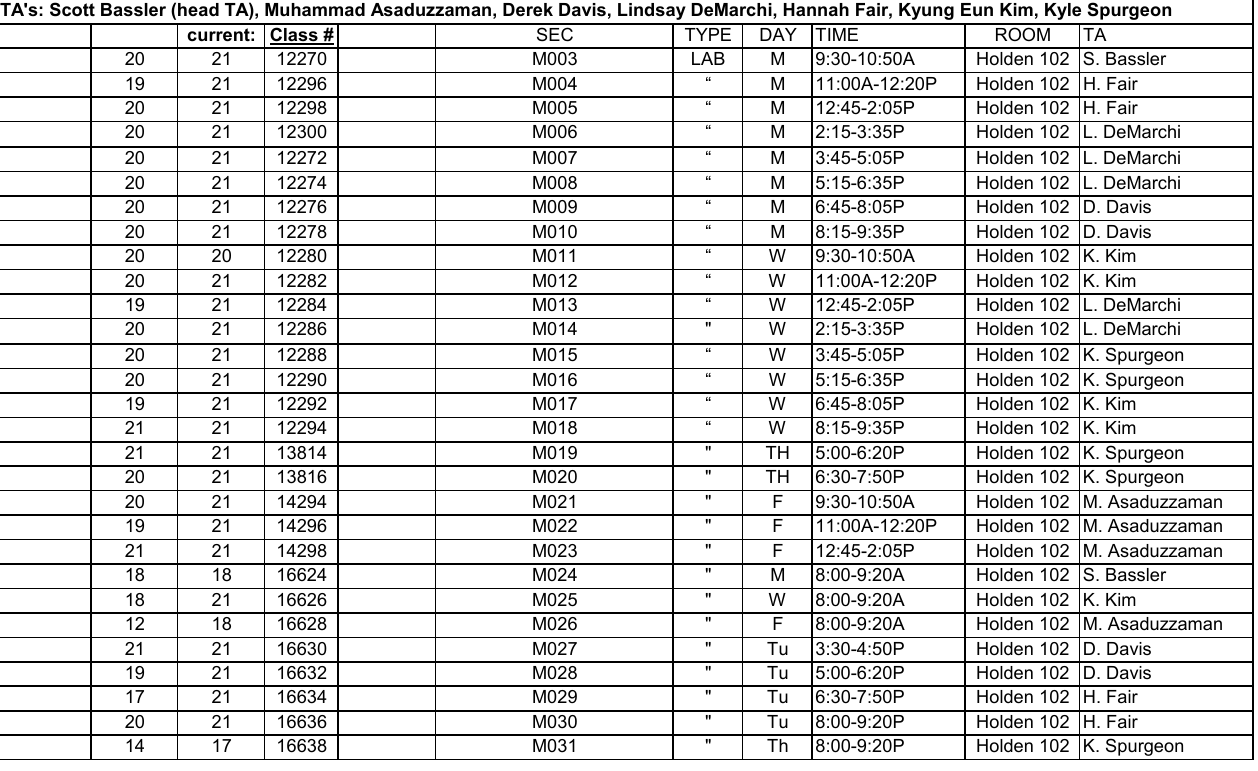
\includegraphics[height=0.9\textheight]{lab-schedule.png}
\EC
\newpage
\Large \centerline{\sc{Reference}}
\normalsize

\begin{center}
Kepler's three laws of orbital motion state:
\end{center}

\BI
\item Planets orbit in ellipses with the Sun at one focus
\item The line connecting a planet to the Sun sweeps out equal areas in equal times
\item The time $T$ required for a planet to orbit the Sun is related to the orbit's semimajor axis $A$ by $T^2 \propto A^3$.
\EI

These laws are equally valid for other gravitationally-bound orbits.

\bigskip
\bigskip
\bigskip

\begin{center}
Newton's three laws of motion state:
\end{center}

\BI
\item An object with no net force acting on it travels in a straight line at a constant velocity.
\item If a force acts on an object, this creates an acceleration on it, with that acceleration given by $F=ma$ or equivalently $a=F/m$.
\item If object A exerts a force on object B, object B exerts an equal force in the opposite direction on object A
\EI

\bigskip
\bigskip
\bigskip

\begin{center}
Newton's law of universal gravitation states:
\end{center}

\BI
\item
The force of gravity between two objects is given by
$$F_g=\frac{Gm_1m_2}{r^2}$$
where $m_1$ and $m_2$ are their masses and $r$ is the distance between their centers.
\EI

\newpage
\normalsize
\begin{enumerate}
% beginning of question comet-orbit-energy
\begin{minipage}{\textwidth}
\item{Consider a comet in the following very eccentric orbit that orbits clockwise:

\BS
\BC
\includegraphics[width=4in]{images/ellipse1-crop.pdf}
\EC
\BS

At which point is the kinetic energy of the comet increasing?

\begin{enumerate}[label=(\Alph*)]
\setlength\itemsep{0.0em}
\item{ Point A }
\item{ Point B }
\item{ Point C }
\item{ Point D }
\item{ Since energy is conserved, the kinetic energy is the same everywhere }
\end{enumerate}
} % end of question comet-orbit-energy
\end{minipage}


\vspace{0.5in}

% beginning of question grav-force-mass
\begin{minipage}{\textwidth}
\item{Suppose I take a large rock (mass 20 kg) and a small rock (mass 10 kg) to the surface of the Moon and drop them from the same height.
How does the {\it gravitational force} on the large rock compare to the gravitational force on the small rock?

\begin{enumerate}[label=(\Alph*)]
\setlength\itemsep{0.0em}
\item{ The gravitational force on the large rock is the same as the gravitational force on the small rock }
\item{ The gravitational force on the large rock is twice as large as the gravitational force on the small rock }
\item{ The gravitational force on the large rock is four times as large as the gravitational force on the small rock }
\item{ In order to figure this out, you also need to know the sizes of the rocks }
\end{enumerate}
} % end of question grav-force-mass
\end{minipage}


\vspace{0.5in}

% beginning of question three-asteroids
\begin{minipage}{\textwidth}
\item{Three asteroids are floating in space as shown. Their masses are given, expressed in arbitrary units,
and the distances separating them are shown, also expressed in arbitrary units.

\bigskip

\begin{center}
\includegraphics[width=0.8\textwidth]{images/three-asteroids.png}
\end{center}

\bigskip

Which asteroid exerts a stronger gravitational force on the asteroid labeled A?

\begin{enumerate}[label=(\Alph*)]
\setlength\itemsep{0.0em}
\item{ The force exerted by asteroids B and C is equal. }
\item{ Asteroid B }
\item{ Asteroid C }
\item{ It is not possible to tell from this picture. }
\end{enumerate}
} % end of question three-asteroids
\end{minipage}


\vspace{0.5in}

% beginning of question four-points-two
\begin{minipage}{\textwidth}
\item{Here is the orbit of the dwarf planet Fido.

\BS
\BC
\includegraphics[width=2in]{images/four-points-crop.pdf}
\EC
\BS

At which shown point is the planet {\it slowing down}? The planet moves counterclockwise in its orbit as seen here. 

\begin{enumerate}[label=(\Alph*)]
\setlength\itemsep{0.0em}
\item{ Point A }
\item{ Point B }
\item{ Point C }
\item{ Point D }
\item{ It is impossible to tell from the figure given }
\end{enumerate}
} % end of question four-points-two
\end{minipage}


\vspace{0.5in}

% beginning of question keplers-laws-apply
\begin{minipage}{\textwidth}
\item{Which object do Kepler's laws {\it not} apply to?

\begin{enumerate}[label=(\Alph*)]
\setlength\itemsep{0.0em}
\item{ Jupiter's moon Ganymede, in its orbit around Jupiter }
\item{ The asteroid 'Oumuamua, which was ejected from another solar system, is flying rapidly through ours, and will soon leave  our solar system again and head to the constellation Pegasus }
\item{ The International Space Station, in its orbit around Earth }
\item{ The dwarf planet Eris, in its orbit around the Sun }
\item{ Kepler's laws apply to all of the above }
\end{enumerate}
} % end of question keplers-laws-apply
\end{minipage}


\vspace{0.5in}

% beginning of question thirdlaw-semimajor
\begin{minipage}{\textwidth}
\item{Suppose an asteroid orbits in a highly eccentric orbit, shaped as shown.

\begin{center}
\includegraphics[width=0.7\textwidth]{images/eccorbit-crop.pdf}
\end{center}

\bigskip

Earth's orbit is nearly circular with a diameter of 2 AU. It has an orbital period of
1 year. Saturn's orbit is nearly circular with a diameter of around 20 AU; it has
an orbital period of around 30 years.

\bigskip

Will this asteroid's orbital period be closest to:

\begin{enumerate}[label=(\Alph*)]
\setlength\itemsep{0.0em}
\item{ 30 years }
\item{ 0.5 year }
\item{ 1 year }
\item{ 15 years }
\end{enumerate}
} % end of question thirdlaw-semimajor
\end{minipage}


\vspace{0.5in}

% beginning of question copernican-advance
\begin{minipage}{\textwidth}
\item{Which is true about the Copernican heliocentric model of the solar system?

\begin{enumerate}[label=(\Alph*)]
\setlength\itemsep{0.0em}
\item{ It is unable to explain the phases of the Moon }
\item{ It is a combination of the old geocentric model and the modern perspective; in it, the Earth orbits the Sun, and all the  planets orbit the Earth }
\item{ It predicts the retrograde motion of the planets without the need for epicycles }
\item{ It gives more accurate predictions than Ptolemy's geocentric model }
\item{ None of the above are true }
\end{enumerate}
} % end of question copernican-advance
\end{minipage}


\vspace{0.5in}

% beginning of question four-points-one
\begin{minipage}{\textwidth}
\item{Here is the orbit of the dwarf planet Fido.

\BS
\BC
\includegraphics[width=2in]{images/four-points-crop.pdf}
\EC
\BS

At which shown point is the planet moving the {\it slowest}?

\begin{enumerate}[label=(\Alph*)]
\setlength\itemsep{0.0em}
\item{ Point A }
\item{ Point B }
\item{ Point C }
\item{ Point D }
\item{ It is impossible to tell from the figure given }
\end{enumerate}
} % end of question four-points-one
\end{minipage}


\vspace{0.5in}

% beginning of question planet-data-table-third-law
\begin{minipage}{\textwidth}
\item{Galileo saw four large moons of Jupiter using a telescope. Here is a table showing how far they are from Jupiter.
\bigskip

\begin{center}
\begin{tabular}{|l|l|}
\hline
Moon  & Distance from Jupiter (km) \\ \hline
Io      & 421,800              \\ \hline
Europa  & 671,100              \\ \hline
Ganymede& 1,070,400           \\ \hline
Callisto& 1,882,700           \\ \hline
\end{tabular}
\end{center}

\bigskip

Which of the following things could be predicted from these data based on Kepler's laws?

\begin{enumerate}[label=(\Alph*)]
\setlength\itemsep{0.0em}
\item{ Io's orbit has the greatest difference between its aphelion and perihelion distance }
\item{ Europa takes longer to orbit Jupiter than Io }
\item{ Callisto is the most massive of these moons }
\item{ Ganymede and Callisto will have more eccentric orbits than Io and Europa }
\item{ None of the above, since Kepler's laws only apply to planets, not moons }
\end{enumerate}
} % end of question planet-data-table-third-law
\end{minipage}


\vspace{0.5in}

% beginning of question boats-on-lake
\begin{minipage}{\textwidth}
\item{Two light boats are floating on the surface of Lake Onondaga. The red boat has three people in it; the green boat has one person in it.
(Assume that all people have the same mass.) The two boats are tied together by a rope.

\BS

The person in the green boat wants to pull the red boat to him. He pulls on the rope; after he pulls, the red boat is moving 
at one meter per second.

\BS

How fast will the green boat be moving right after this happens?

\begin{enumerate}[label=(\Alph*)]
\setlength\itemsep{0.0em}
\item{ It won't be moving at all }
\item{ 1 meter per second }
\item{ 1/3 meter per second }
\item{ 3 meters per second }
\end{enumerate}
} % end of question boats-on-lake
\end{minipage}


\vspace{0.5in}

% beginning of question ellipse-shape-discovery
\begin{minipage}{\textwidth}
\item{Which advance in astronomy led {\it most directly} to the discovery that the planets travel in elliptical orbits?

\begin{enumerate}[label=(\Alph*)]
\setlength\itemsep{0.0em}
\item{ The precision measurements of the positions of the planets in the sky made by Tycho, Sophie, and Kepler }
\item{ The observation of Jupiter's moons through a telescope made by Galileo }
\item{ The discovery of the mathematical form of the law of gravity by Isaac Newton }
\item{ The correction of mathematical errors in the {\it Almagest} made by Islamic mathematicians }
\item{ The realization that retrograde motion could be easily explained by a heliocentric model by Copernicus }
\end{enumerate}
} % end of question ellipse-shape-discovery
\end{minipage}


\vspace{0.5in}

% beginning of question gravity-properties
\begin{minipage}{\textwidth}
\item{Which of the following is {\it incorrect} about Newton's law of gravitation? {\it (Thanks to Kim for the question!)}

\begin{enumerate}[label=(\Alph*)]
\setlength\itemsep{0.0em}
\item{ Doubling the mass of one object doubles the force of gravity between the two objects	 }
\item{ The strength of the gravitational force attracting any two objects is {\it inversely} proportional to the product of their masses. }
\item{ The strength of the gravitational force between two objects decreases with the square of the distance between their centers }
\item{ Every object in the Universe attracts every other mass  }
\item{ Doubling the distance between two objects weakens the force of gravity by a factor of $2^2$ or 4. }
\end{enumerate}
} % end of question gravity-properties
\end{minipage}


\vspace{0.5in}

% beginning of question grav-accel-mass
\begin{minipage}{\textwidth}
\item{Suppose I take a large rock (mass 20 kg) and a small rock (mass 10 kg) to the surface of the Moon and drop them from the same height.
How does the {\it acceleration due to gravity} on the large rock compare to the acceleration due to gravity on the small rock?

\begin{enumerate}[label=(\Alph*)]
\setlength\itemsep{0.0em}
\item{ The gravitational acceleration on the large rock is twice as large as the gravitational acceleration on the small rock }
\item{ The gravitational acceleration on the large rock is four times as large as the gravitational acceleration on the small rock }
\item{ The gravitational acceleration on the large rock is the same as the gravitational acceleration on the small rock }
\item{ In order to figure this out, you also need to know the mass of the Moon }
\end{enumerate}
} % end of question grav-accel-mass
\end{minipage}


\vspace{0.5in}

% beginning of question four-points-three
\begin{minipage}{\textwidth}
\item{Here is the orbit of the dwarf planet Fido.

\BS
\BC
\includegraphics[width=2in]{images/four-points-crop.pdf}
\EC
\BS

At which point does Fido have the largest {\it total energy}? {\it (Thanks to Landon for the question!)}

\begin{enumerate}[label=(\Alph*)]
\setlength\itemsep{0.0em}
\item{ Point A }
\item{ Point B }
\item{ Point C }
\item{ Point D }
\item{ The total energy is the same at all of the points shown. }
\end{enumerate}
} % end of question four-points-three
\end{minipage}


\vspace{0.5in}

% beginning of question earth-round-discovery
\begin{minipage}{\textwidth}
\item{Who first discovered that the Earth was spherical?

\begin{enumerate}[label=(\Alph*)]
\setlength\itemsep{0.0em}
\item{ Nikolaus Copernicus }
\item{ Isaac Newton }
\item{ Christopher Columbus }
\item{ Galileo Galilei }
\item{ None of the above; the Earth was known to be round thousands of years prior to the Renaissance. }
\end{enumerate}
} % end of question earth-round-discovery
\end{minipage}


\vspace{0.5in}

% beginning of question universal-gravitation-consequence
\begin{minipage}{\textwidth}
\item{Which of the following {\it is} explained by Isaac Newton's laws of universal gravitation and mechanics, but {\it not} explained
by Kepler's laws of orbital motion?

\begin{enumerate}[label=(\Alph*)]
\setlength\itemsep{0.0em}
\item{ The fact that Mercury appears to move backwards in the sky periodically }
\item{ The fact that the more distant moons of Jupiter take longer to go around than the closer moons }
\item{ The fact that Halley's comet spends most of its time far from the Sun, and is only close enough to the Sun for us to see it for a tiny fraction of each orbit }
\item{ The fact that Earth is closer to the Sun during December than during June }
\item{ The slight motion of the Sun due to Jupiter's gravity }
\end{enumerate}
} % end of question universal-gravitation-consequence
\end{minipage}


\vspace{0.5in}

% beginning of question galilean-moons-consequence
\begin{minipage}{\textwidth}
\item{Galileo observed four moons orbiting Jupiter through the first astronomical telescope. What did he deduce from this?

\begin{enumerate}[label=(\Alph*)]
\setlength\itemsep{0.0em}
\item{ That the orbits of these moons are elliptical, not circular }
\item{ That the motion of these moons can only be explained using ``epicycles'' }
\item{ That not everything orbits the Earth }
\item{ That Jupiter's gravity gets weaker the further out you are from it, leading to the later discovery of Kepler's third law }
\item{ More than one of the above }
\end{enumerate}
} % end of question galilean-moons-consequence
\end{minipage}


\vspace{0.5in}

% beginning of question eccentric-energy
\begin{minipage}{\textwidth}
\item{Here are some pairs of plots for kinetic and gravitational potential energy.
Which one represents the fluctuation of KE and GPE for a planet in a
strongly eccentric orbit, like Halley's comet?

\begin{enumerate}[label=(\Alph*)]
\setlength\itemsep{0.0em}
\item{ \raisebox{-.5\height}{\includegraphics[width=0.4\textwidth]{images/PE-earthlike-crop.pdf}} \hspace{0.05\textwidth} \raisebox{-.5\height}{\includegraphics[width=0.4\textwidth]{images/KE-earthlike-crop.pdf}} }
\item{ \raisebox{-.5\height}{\includegraphics[width=0.4\textwidth]{images/PE-ecc15offset-crop.pdf}} \hspace{0.05\textwidth} \raisebox{-.5\height}{\includegraphics[width=0.4\textwidth]{images/KE-ecc15offset-crop.pdf}} }
\item{ \raisebox{-.5\height}{\includegraphics[width=0.4\textwidth]{images/PE-earthoffset-crop.pdf}} \hspace{0.05\textwidth} \raisebox{-.5\height}{\includegraphics[width=0.4\textwidth]{images/KE-earthoffset-crop.pdf}} }
\item{ \raisebox{-.5\height}{\includegraphics[width=0.4\textwidth]{images/PE-ecc16-crop.pdf}} \hspace{0.05\textwidth} \raisebox{-.5\height}{\includegraphics[width=0.4\textwidth]{images/KE-ecc16-crop.pdf}} }
\end{enumerate}
} % end of question eccentric-energy
\end{minipage}


\vspace{0.5in}

% beginning of question kepler-third-evidence
\begin{minipage}{\textwidth}
\item{An astronaut is doing a ``spacewalk'' to repair the International Space Station, in orbit 250 miles (400 km) above the surface of the
Earth. They float next to it without needing to hold on 
tightly. What principle of physics causes the astronaut to stay
next to the Space Station?

\begin{enumerate}[label=(\Alph*)]
\setlength\itemsep{0.0em}
\item{ According to Kepler's second law of orbital motion, the astronaut and the Space Station orbit around the same point. }
\item{ According to Newton's first law of motion, objects in motion stay in motion in a straight line without an external force acting on them. Both the the Space Station and the astronaut are in motion, and without external forces acting on them, they will keep moving together. }
\item{ According to Newton's law of universal gravitation, the Earth's gravitational force is equal on the astronaut and the Space  Station, causing them to move together. }
\item{ According to Newton's law of universal gravitation, the astronaut and the Space Station are so far away from Earth that Earth's  gravity doesn't really affect them }
\item{ According to Kepler's third law of orbital motion, the astronaut must have the same orbital period as the Space Station, since they are in the same orbit, even though the Space Station is much more massive. }
\end{enumerate}
} % end of question kepler-third-evidence
\end{minipage}


\vspace{0.5in}

% beginning of question planet-data-table-second-law
\begin{minipage}{\textwidth}
\item{Here is a table showing the orbital distances, orbital periods, and masses for the six planets known in Kepler's time. Jupiter is the most massive of these planets, and Mercury is the least.

\bigskip

\begin{center}
\begin{tabular}{|l|l|l|l|l|}
\hline
Planet  & Semimajor axis (AU) & Orbital period (years) & Mass (Earths) & Eccentricity \\ \hline
Mercury & 0.38                & 0.24                   & 0.06                          & 0.206  \\ \hline
Venus   & 0.72                & 0.61                   & 0.81                          & 0.007  \\ \hline
Earth   & 1.0                 & 1.0                    & 1.0                           & 0.017  \\ \hline
Mars    & 1.52                & 1.88                   & 0.11                          & 0.093  \\ \hline
Jupiter & 5.20                & 11.86                  & 318                           & 0.048  \\ \hline
Saturn  & 9.54                & 29.46                  & 95.2                          & 0.054  \\ \hline
\end{tabular}
\end{center}

\bigskip

Of these objects, which one has the {\it greatest percent change} in its speed over the course of one orbit around the Sun?

\begin{enumerate}[label=(\Alph*)]
\setlength\itemsep{0.0em}
\item{ Mercury }
\item{ Venus }
\item{ Jupiter }
\item{ Saturn }
\item{ The speed of planets does not change as they orbit the Sun. }
\end{enumerate}
} % end of question planet-data-table-second-law
\end{minipage}


\vspace{0.5in}

% beginning of question parallax-two
\begin{minipage}{\textwidth}
\item{{\it Parallax} is the apparent motion of an object against the background when the observer changes location. The {\it baseline}
is the distance that the observer moves.

Which combination of factors will produce the largest observed parallax?

\begin{enumerate}[label=(\Alph*)]
\setlength\itemsep{0.0em}
\item{ A short baseline when observing a distant object }
\item{ A short baseline when observing a nearby object }
\item{ A long baseline when observing a nearby object }
\item{ A long baseline when observing a distant object }
\end{enumerate}
} % end of question parallax-two
\end{minipage}


\vspace{0.5in}

% beginning of question find-sun-secondlaw
\begin{minipage}{\textwidth}
\item{An asteroid orbits the Sun in an orbit like the one shown below.
\BS
\BC
\includegraphics[width=3in]{images/secondlaw-ellipse-crop.pdf}
\EC
\BS
This asteroid takes ten months to make one complete orbit. Its position after each month is indicated, \ie the labeled points are
located one month apart.

Which position is the correct position of the Sun? 

\begin{enumerate}[label=(\Alph*)]
\setlength\itemsep{0.0em}
\item{ Position A }
\item{ Position B }
\item{ Position C }
\item{ There's isn't enough information given to know for sure }
\end{enumerate}
} % end of question find-sun-secondlaw
\end{minipage}


\vspace{0.5in}

% beginning of question grav-force-distance-easy
\begin{minipage}{\textwidth}
\item{Suppose that a new planet Twilo is added to the Solar System. Twilo has the same size and mass as Earth, but is located in a circular
orbit 5 AU from the Sun.

\BS

Which of the following is true about the gravitational force the Sun exerts on Twilo?

\begin{enumerate}[label=(\Alph*)]
\setlength\itemsep{0.0em}
\item{ The gravitational force that the Sun applies to Twilo is 1/25 as strong as the gravitational force that the Sun applies to Earth. }
\item{ The gravitational force that the Sun applies to Twilo is 25 times stronger as the gravitational force that the Sun appplies to Earth.  }
\item{ The gravitational force that the Sun applies to Twilo is 5 times stronger than the gravitational force that the Sun applies to Earth. }
\item{ The gravitational force that the Sun applies to Twilo is 1/5 as strong as the gravitational force that the Sun applies to Earth. }
\item{ The gravitational force that the Sun applies to Twilo is the same size as the gravitational force that the Sun applies to Earth.  }
\end{enumerate}
} % end of question grav-force-distance-easy
\end{minipage}


\vspace{0.5in}

% beginning of question gravity-strength
\begin{minipage}{\textwidth}
\item{A spacecraft is floating halfway between the Earth and the Moon. Which object exerts a larger force on the spacecraft? {\it (Thanks to Jen for the question!)}

\begin{enumerate}[label=(\Alph*)]
\setlength\itemsep{0.0em}
\item{ The spacecraft exerts a force on the planets, not the other way around. }
\item{ The Moon }
\item{ Both exert the same force on the spacecraft.	 }
\item{ There is not enough information for us to tell.	 }
\item{ The Earth }
\end{enumerate}
} % end of question gravity-strength
\end{minipage}


\vspace{0.5in}

% beginning of question grav-force-combination
\begin{minipage}{\textwidth}
\item{Suppose a person weighs 120 pounds on the surface of the Earth. That means that the force of Earth's gravity on her is 120 pounds.

\BS

If she travels to the Moon, the strength of the Moon's gravitational force on her will be only about 20 pounds -- that is,
the Moon's gravity on its surface is 1/6 as strong as Earth's gravity on its surface.

\BS

The mass of the Moon is about 1/96 of the mass of the Earth.

\BS

The radius of the Moon is most nearly:

\begin{enumerate}[label=(\Alph*)]
\setlength\itemsep{0.0em}
\item{ 1/2 the radius of the Earth }
\item{ 1/4 the radius of the Earth }
\item{ 1/96 the radius of the Earth }
\item{ 1/36 the radius of the Earth }
\item{ 1/6 the radius of the Earth }
\end{enumerate}
} % end of question grav-force-combination
\end{minipage}


\vspace{0.5in}

% beginning of question parallax
\begin{minipage}{\textwidth}
\item{What is true regarding the lack of observed parallax in the distant stars when we look at them first in the 
summer and then in the winter?

\begin{enumerate}[label=(\Alph*)]
\setlength\itemsep{0.0em}
\item{ Because a baseline of 2 AU is too small to observe parallax with the unaided eye, since the stars are so far away }
\item{ We actually {\it do} observe parallax in the distant stars when observing them with modern instruments }
\item{ The lack of observed parallax was a piece of evidence used to argue that the Earth could not move }
\item{ If we did observe parallax in the stars, we could use it to figure out how far away they are }
\item{ All of the above are true }
\end{enumerate}
} % end of question parallax
\end{minipage}


\vspace{0.5in}

% beginning of question comet-potential-energy
\begin{minipage}{\textwidth}
\item{Consider the highly eccentric orbit of a comet shown below.

\BS

\BC
\includegraphics[width=4in]{images/ellipse1-crop.pdf}
\EC

\BS

At which labeled point does the comet have the most {\it potential energy}? 

\begin{enumerate}[label=(\Alph*)]
\setlength\itemsep{0.0em}
\item{ Point A }
\item{ Point B }
\item{ Point C }
\item{ Point D }
\end{enumerate}
} % end of question comet-potential-energy
\end{minipage}


\vspace{0.5in}

% beginning of question keplers-third-law-twilo
\begin{minipage}{\textwidth}
\item{Suppose that a new planet Twilo is added to the Solar System. Twilo has the same size and mass as Earth, but is located in a circular
orbit 5 AU from the Sun.

\bigskip

Which of the following is true about Twilo? 

\begin{enumerate}[label=(\Alph*)]
\setlength\itemsep{0.0em}
\item{ Twilo takes between one year and five year to orbit the Sun. }
\item{ Twilo takes less than one year to orbit the Sun. }
\item{ Twilo takes more than five years to orbit the Sun. }
\item{ Twilo orbits the Sun in one year. }
\item{ Twilo orbits the Sun in five years. }
\end{enumerate}
} % end of question keplers-third-law-twilo
\end{minipage}


\vspace{0.5in}

% beginning of question earth-inflate
\begin{minipage}{\textwidth}
\item{Suppose that someone weighs 180 pounds. {\it (``Weight'' refers to the force of gravity on an object.)}

If Earth's size were increased by a factor of three, while keeping its mass the same, how much would they then weigh?

\begin{enumerate}[label=(\Alph*)]
\setlength\itemsep{0.0em}
\item{ 60 pounds }
\item{ 180 pounds }
\item{ 1,620 pounds }
\item{ 20 pounds }
\item{ 540 pounds }
\end{enumerate}
} % end of question earth-inflate
\end{minipage}


\vspace{0.5in}

\end{enumerate}
\newpage\Large\sc\BC Scratch Paper\EC
\newpage\Large\sc\BC Scratch Paper\EC
\newpage
\end{document}
